\documentclass[a4paper, 11pt]{article}
\usepackage{geometry}
\geometry{letterpaper, margin=1in}
\usepackage{amsmath}
\usepackage{amssymb}  
\usepackage{amsthm}
\usepackage{ulem} 
\usepackage{graphicx}
\graphicspath{ {images/} }

\begin{document}
%Header-Make sure you update this information!!!!
\noindent
\large\textbf{Homework 3} \hfill \textbf{John Waczak} \\
\normalsize PH 431 \hfill  Date: \today \\
Prof. Bo Sun  \\
Worked with: Katy Chase, Daniel Still, Cassandra H. \\


\section*{1. Dielectric Image Charges}

\textit{2 Dielectric materials $\epsilon_1, \epsilon_2$ meet at an infinitely big, flat surface. A free charge $q_f$ is placed a distance d from the surface. What is the electric field in each of the materials?}\\ 

\noindent In order to solve this problem we need to identify some boundary conditions that will come in handy for defining the potential in each half of the material. Recall that from the definition of the displacement field in a linearly polarized material we have $\nabla \cdot \mathbf{D} = \rho_f$. We can rewrite this as a condition on the electric field above and below the interface (which we set here to be $z=0$). 
	\begin{align*}
		\mathbf{D} &= \epsilon \mathbf{E} \\
		\nabla \cdot \mathbf{D} &= \nabla \cdot \epsilon \mathbf{E} = \rho_f \\ 
		\Rightarrow \text{BC's} &
		\begin{cases}
			\nabla \cdot \mathbf{E} = \frac{\rho_f}{\epsilon}, & z > 0 \\ 
			\nabla \cdot \mathbf{E} = 0, & z < 0 \\
		\end{cases}
	\end{align*}
Furthermore, we have that the perpendicular component of the \textbf{D} field must be continuous across the interface as well as the potential. This translates into the following mathematical expressions: 
	\begin{align}
		\phi_{a}(z=0) &= \phi_{b}(z=0) \\ 
		\epsilon_1 \frac{\partial \phi_a}{\partial z} \Big|_{z=0} &= \epsilon_2 \frac{\partial \phi_b}{\partial z} \Big|_{z=0} 
	\end{align}
Where here we use a and b to mean above and below. To solve for the electric field in both regions, we will employ the method of images in order to determine candidates for $\phi_a, \phi_b$. We will then show that these equations satisfy boundary conditions 1 and 2 as well as Poisson and Laplace's equations in each reason in order to invoke the uniqueness theorem. \\ 

\noindent First, let's consider the following problem which I claim will produce the same scalar potential above the interface. 
		\begin{center}
			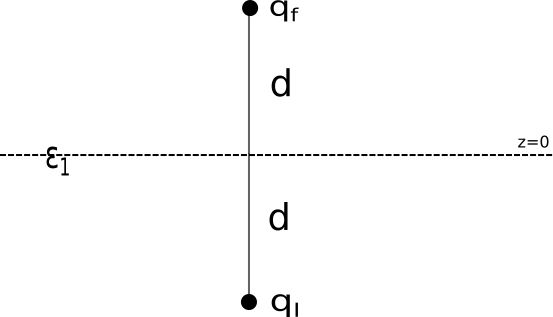
\includegraphics[scale=0.5]{fig1}
		\end{center}
For this system, I am considering only one dielectric of $\epsilon_1$ with an image charge placed the same distance d below the $z=0$ axis. Now clearly this system will satisfy $\nabla \cdot \mathbf{E} = \rho_f/\epsilon$ for $z > 0$ because the only charge in that region is the original free charge. Thus a Gaussian sphere would quickly verify this condition holds. 	Because these are point charges in a linearly dielectric material, we can quickly write down the potential at a point above $z=0$ as: 
	\begin{equation}
		\phi_a(x,y,z>0) = \frac{1}{4\pi\epsilon_0\epsilon_1}\Bigg[ \frac{q_f}{\sqrt{x^2+y^2+(z-d)^2}}+ \frac{q_I}{\sqrt{x^2+y^2+(z+d)^2}}\Bigg] 
	\end{equation}
	
\noindent Now to find $\phi_b$ let's consider a second image charge situation illustrated in the following diagram. \\
	\begin{center}
		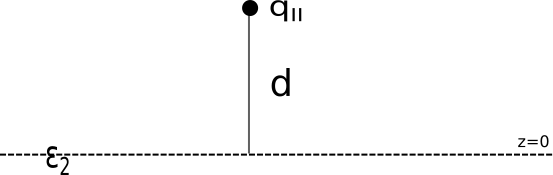
\includegraphics[scale=0.5]{fig2}
	\end{center}
	
\noindent Here we are considering a single dielectric of $\epsilon_2$ with some unknown charge $q_{II}$ placed a distance d above $z=0$. This system clearly satisfies $\nabla \cdot \mathbf{E} = 0$ in the region $z<0$ because there is \textit{no} charge in that region. Once again we can easily write down the potential at a position below the $z=0$ line as follows: 
	\begin{equation}
		\phi_b(x,y,z<0) = \frac{1}{4\pi\epsilon_0\epsilon_1}\frac{q_{II}}{\sqrt{x^2+y^2+(z-d)^2}}
	\end{equation}
Now all that remains to do is fit $q_I, q_{II}$ to boundary conditions 1 and 2. Let's start with condition 1. Evaluating both functions at $z=0$ gives: 	
	\begin{align*}
		\frac{1}{4\pi\epsilon_0\epsilon_1}\frac{q_f+q_{I}}{\sqrt{x^2+y^2+d^2}} &= \frac{1}{4\pi\epsilon_0\epsilon_2}\frac{q_{II}}{\sqrt{x^2+y^2+d^2}} \\ 
		\Rightarrow \frac{1}{\epsilon_1}[q_f + q_I] &= \frac{1}{\epsilon_2}[q_{II}]
	\end{align*}
\noindent Now applying 2 requires taking derivatives with respect z which I did using Mathematica (see attached code). 
	\begin{align*}
		\epsilon_1\frac{\partial \phi_a}{\partial z} &= \frac{1}{4\pi\epsilon_0}\Bigg[ \frac{-(d+z)q_I}{(x^2+y^2+(d+z)^2)^{3/2}} + \frac{-(z-d)q_{f}}{(x^2+y^2+(z-d)^2)^{3/2}}\Bigg] \\ 
		\epsilon_2\frac{\partial \phi_b}{\partial_z} &= \frac{1}{4\pi\epsilon_0}\Bigg[\frac{-(z-d)q_{II}}{(x^2+y^2+(z-d)^2)^{3/2}}\Bigg]
	\end{align*}
Evaluating at $z=0$ gives: 
	\begin{equation*}
		q_{II} = q_f-q_I
	\end{equation*}
Now we simply need to solve the following system: 
	\begin{equation}
		\begin{cases}
			 \frac{1}{\epsilon_1}[q_f + q_I] = \frac{1}{\epsilon_2}[q_{II}] \\
			 q_{II} = q_f-q_I
		\end{cases}
	\end{equation}
	
	\begin{align*}
		\frac{1}{\epsilon_1}(q_f+q_I) &= \frac{1}{\epsilon_2}(q_f - q_I) \\ 
		\frac{\epsilon_2}{\epsilon_1}q_f + \frac{\epsilon_2}{\epsilon_1}q_I &= q_f - q_I \\ 
		q_I &= q_f \Bigg( \frac{1-\frac{\epsilon_2}{\epsilon_1}}{1+\frac{\epsilon_2}{\epsilon_1}}\Bigg) \\
		q_{II} &= q_f - q_f \Bigg( \frac{1-\frac{\epsilon_2}{\epsilon_1}}{1+\frac{\epsilon_2}{\epsilon_1}}\Bigg)
	\end{align*}
And so after some simplification we conclude that: 
	\begin{align}
		q_I &= -q_f \Bigg( \frac{\epsilon_2-\epsilon_1}{\epsilon_2+\epsilon_1}\Bigg) \\ 
		q_{II} &= q_f \Bigg( \frac{2\epsilon_2}{\epsilon_1+\epsilon_2} \Bigg)
	\end{align}
By equations 6 and 7 we force our potential to meet the necessary boundary conditions. Thus the full definition for $\phi$ can be written as: 
	\begin{equation}
		\phi(x,y,z) = 
		\begin{cases}
			\frac{1}{4\pi\epsilon_0\epsilon_1}\Bigg[ \frac{q_f}{\sqrt{x^2+y^2+(z-d)^2}}+ \frac{-q_f\Big( \frac{\epsilon_2-\epsilon_1}{\epsilon_2+\epsilon_1}\Big)}{\sqrt{x^2+y^2+(z+d)^2}}\Bigg] & z > 0 \\ 
			\frac{1}{4\pi\epsilon_0\epsilon_2}\Bigg[ \frac{q_f\Big(\frac{2\epsilon_2}{\epsilon_1+\epsilon_2}\Big)}{\sqrt{x^2+y^2+(z-d)^2}}\Bigg] & z<0
		\end{cases}
	\end{equation}
The electric field is simply the gradient of the potential $\nabla \phi$ which is shown at the bottom of the following Mathematica code in terms of the x, y, and z components of the field. Above is labeled with a 1 and below is labeled with a 2. 
	\begin{center}
		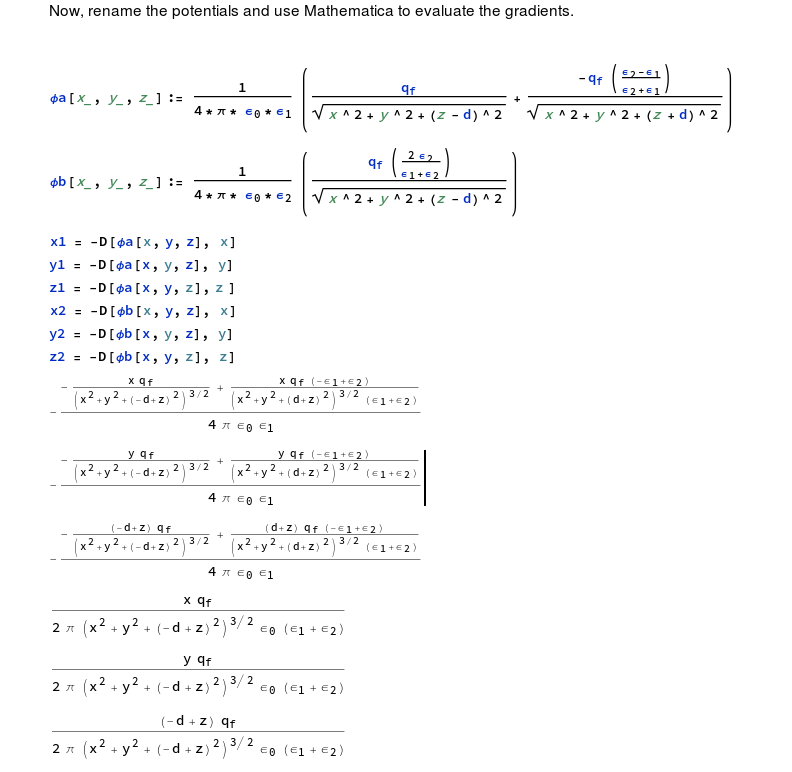
\includegraphics[scale=.69]{code2}
	\end{center}
	
\section*{2. Capacitor with non-uniform dielectric}
\textit{A capacitor is formed by two parallel plates of area A in the z direction. One sits at $z=0$ and the other sits at $z=h$. The plates have +Q and -Q respectively and are filled with a linear dielectric constant of $\epsilon = \epsilon_0 + \alpha z$. Assuming the plates are large 1) find the bound charge distribution in the capacitor, 2) calculate the total energy stored in the capacitor. }\\ 

\noindent Recall the law for linearly dielectric materials: $\nabla \cdot \mathbf{D} = \rho_f$. In order to determine \textbf{D} we will take an infinitesimally thin Gaussian pillbox around the top plate of the capacitor. We can make the box thin enough so that all of the flux of \textbf{D} goes through the top and bottom surfaces. Thus we have: 
	\begin{align*}
		\oint\limits_S \mathbf{D} \cdot d\mathbf{s} &= Q \\ 
		-\mathbf{D}_{in}A + \mathbf{D}_{out}  &= Q \\
		\Rightarrow \mathbf{D}_{in} &= -\frac{Q}{A} \hat{z} 
	\end{align*}
The last line follows because if we treat the plates as if they are infinite we have the result from electrostatics that the electric field must be zero outside the capacitor due to superposition and $\mathbf{D} = \epsilon\mathbf{E}$. Now that we have \textbf{D} we can solve for the dipole moment density and then subsequently the surface bound charge and volume bound charge. \\ 

\noindent By definition of the displacement field we have: 
	\begin{align*}
		\mathbf{D} &= \epsilon_0 \mathbf{E} + \mathbf{P} \\ 
		\mathbf{D} &= \epsilon \mathbf{E} \\ 
		\Rightarrow \mathbf{P} &= \mathbf{E}(\epsilon - \epsilon_0) \\ 
		&= \mathbf{E}(\epsilon_0 + \alpha z - \epsilon_0) = \alpha z \mathbf{E} \\
		\mathbf{E} &= \mathbf{D}/\epsilon = \frac{-Q}{A(\epsilon_0 + \alpha z)}\hat{z} \\
		\Rightarrow \mathbf{P} &= \frac{-Q\alpha z}{A(\epsilon_0 + \alpha z)}\hat{z}
	\end{align*}
Now that we have \textbf{P}, we can calculate $\sigma_b, \rho_b$. 
	\begin{align*}
		\sigma_b &= \mathbf{P} \cdot \hat{n} \\ 
		&= \begin{cases}
			0; & z=0 \\ 
			\frac{-Q\alpha h}{A(\epsilon_0 + \alpha h)}; & z = h
		\end{cases}\\
		\rho_b &= -\nabla \cdot \mathbf{P} \\
		&= -\frac{\partial}{\partial z}\frac{-Q\alpha z}{A(\epsilon_0 + \alpha z)} \\ 
		&= \frac{Q\alpha}{A}\Bigg[ \frac{1}{\epsilon_0 + \alpha z} + \frac{-\alpha z}{(\epsilon_0 + \alpha z)^2} \Bigg] \\ 
		&= \frac{Q\alpha \epsilon_0}{A(\epsilon_0 + \alpha z)^2}
	\end{align*}

Thus we have found the bound charge density. Now to solve for the energy of the configuration we can equivalently calculate the work required to make the configuration. This equation is given by: 
	\begin{align*}
		W &= \frac{1}{2} \int \mathbf{D} \cdot \mathbf{E} \quad d\tau \\ 
		&= \frac{1}{2} \int \epsilon \mathbf{E}^2 \quad d\tau \\ 
		&= \frac{A}{2} \int\limits_0^h \epsilon \mathbf{E}^2 dz \\ 
		&= \frac{A}{2} \int\limits_0^h \frac{Q^2(\epsilon_0+\alpha z)}{A^2(\epsilon_0 + \alpha z)^2} dz \\
		&= \frac{Q^2}{2A}\int\limits_0^h \frac{1}{\epsilon_0 + \alpha z} dz \\
		&= \frac{Q^2}{2A\alpha}\ln\Big(\frac{\epsilon_0 + \alpha h}{\epsilon_0}\Big)
	\end{align*}

\section*{3 Electromagnetic forces}	
\textit{Two spherical conductors of radius (a) a distance (d) apart are both charged with Q and rotate along their axis at some angular speed $\omega$. What is the ratio between the electric and magnetic interaction forces?}\\ 

\noindent We can estimate this ratio fairly easily up to a pre-factor using dimensional analysis provided that $d >> a$. By taking a Gaussian sphere of radius r around one of the spheres it is easy to see that: 	
	\begin{equation*}
		\mathbf{E} = \frac{Q}{4\pi\epsilon_0 r^2} \quad \quad r>a 
	\end{equation*}
This makes sense as we know from far away a charged sphere behaves like a dipole. Therefore the magnitude of the electric interaction force at a distance d is given by: 
	\begin{equation}
		\mathbf{F}_E = \frac{Q^2}{4\pi\epsilon_0 d^2}
	\end{equation}
	
Now, notice that if we look at a slice of one of the rotating spheres through the plane perpendicular to it's axis of rotation we have some current (I) going in a loop which I will denote counter-clockwise without loss of generality. Because the full sphere is just a series of these loops with varying radius at far field we expect the magnetic field to be that of a magnetic dipole. By direct analogy from electric dipoles, we have that: 
	\begin{equation*}
		\mathbf{F}_B \propto \frac{1}{r^4}
	\end{equation*}
	
Our goal now is to determine the constants necessary to make the dimension of this equation a force. We can expect a factor of $\mu_0$ to appear from the \textbf{B} field which itself has dimensions of $\frac{|\text{Force}|}{|\text{charge}|^2/|\text{time}|^2}$. Thus we can include a factor of $a^4$ to cancel the dimensions of the $d^4$ and adding a $Q^2\omega^2$ finishes the equation i.e. 
	\begin{equation*}
		\mathbf{F}_B \approx \frac{Q^2\omega^2\mu_0 a^4}{d^4}
	\end{equation*}
	
Taking the ratio of the two  magnitudes gives: 
	\begin{align*}
		\frac{F_E}{F_B} &\approx \frac{\Bigg(\frac{Q^2}{4\pi\epsilon_0 d^2}\Bigg)}{\Bigg(\frac{Q^2\omega^2\mu_0 a^4}{d^4}\Bigg)} \\
		&= \frac{Q^2}{4\pi\epsilon_0 d^2} \cdot \frac{d^4}{Q^2\omega^2\mu_0 a^4} \\ 
		&= \frac{d^2}{4\pi\epsilon_0\mu_0\omega^2a^4} \\ 
		&= \frac{c^2d^2}{4\pi\omega^2a^4}
	\end{align*}
Where c is the speed of light. This is dimensionless as desired because the top is a velocity squared and the rest of the terms cancel to give a denominator of velocity squared! Thus we have found the approximate ratio of the electric to the magnetic interaction force. 
\end{document}





























